\documentclass[aspectratio=169]{beamer}
\hypersetup{pdfpagemode=FullScreen}
\usetheme[progressbar=frametitle]{metropolis}
\usepackage{appendixnumberbeamer}
\usepackage{listings}
\bibliographystyle{plainnat}
\usepackage{listings}
\usepackage{hyperref}
\usepackage{booktabs}
\usepackage{tikz}
\usepackage{tikzpeople}
\usepackage{biblatex}
\addbibresource{references.bib}
\usetikzlibrary{shapes,arrows}
\usepackage[scale=1]{ccicons}
% \usepackage{enumitem} % not compatible with enumerate in beamer class
\usepackage{xspace}
\newcommand{\themename}{\textbf{\textsc{metropolis}}\xspace}

\title{Competition}
% \subtitle{Subtítulo}
% \date{\today}
\date{May 30, 2022}
\author{Tensorboys}
\institute{Pattern Recognition}
% \titlegraphic{\hfill\includegraphics[height=1.5cm]{logo.pdf}}

\begin{document}

\maketitle

\begin{frame}{Agenda}
    \setbeamertemplate{section in toc}[sections numbered]
    \tableofcontents
\end{frame}
\section{Multi-layer Perceptron}
\begin{frame}[t]
    \frametitle{MLP}
    \begin{columns}
        \column{0.3\textwidth}

        \begin{itemize}
            \item We've tested multiple architecture from $784\times 2 \times 10$ to $784\times 512 \times 512\times 256 \times 128 \times 10$.
            \item This process was obviously automated.
            \item This yielded interesting results.
        \end{itemize}
        \column{0.7\textwidth}
        \begin{figure}[ht!]
            \centering
            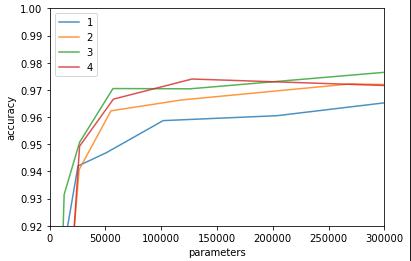
\includegraphics[width=0.7\textwidth]{figures/mlp_layers.png}
            \caption{Relation between parameters and accuracy for different model layers. The number of epochs is 20 and the batch size 128 for each of the model. The best accuracy is 0.9775 with a 3-layer model: $784\times512\times512\times256\times10$.}
            \label{fig:}
        \end{figure}
    \end{columns}
\end{frame}
\section{Convolutional Neural Network}
\end{document}
